\subsection{The 3morduc platform}
\label{sec:3morduc}

\begin{figure} [h]
  \begin{center}
    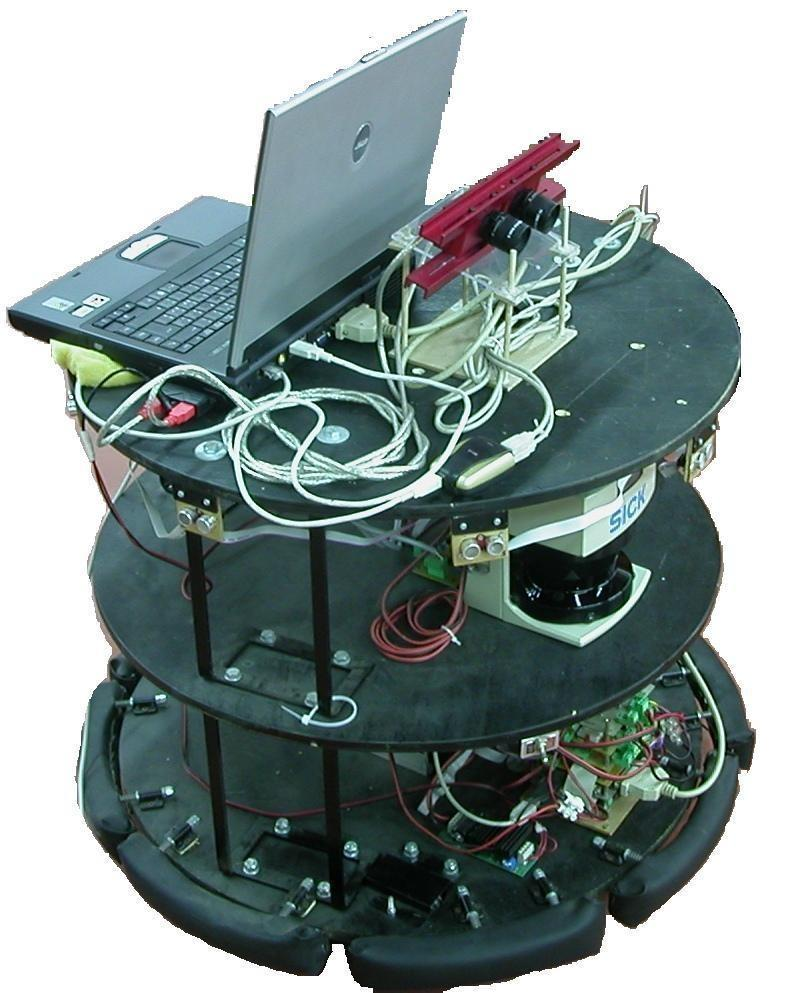
\includegraphics[width=150pt]{img/3morduc.jpg}
    \caption{The 3morduc robotic platform}
    \label{fig:morduc}
  \end{center}
\end{figure}

The telerobot used to develop teleoperation research is
called \textit{3MO.R.D.U.C.}, acronym for `3rd version of
the Mobile Robot DIEES University of Catania'.
3morduc is a mobile-robot, able to move forward, backward
and turn its direction, as directed by the remote operator.
It has been successfully used in several test and experimental
work regarding teleoperation and telepresence.
\\
The robot, actually located at the University of
Catania, is a differential-driven mobile robot, showed
in figure \ref{fig:morduc}.
\\
As every mobile robot, it is equipped with some internal
and external sensors, through which is possible retrieve
information about, respectively, the status of the robot
(e.g. its position) or the data about the environment (e.g.
distance from obstacles).

\subsubsection{Sensors and actuators}
\label{sec:3morduc:sensors_actuators}


The moviment is performed by means of two 40W DC engines, model
\textit{Maxon F2260}, connected with the motor shaft by a gear
box (transmission rate 1/19). On the other side the motor shaft
is linked with two rubber wheels, while a third castor wheel can
freely turn to realize the differential-driven model.
\\
The robot is compound by three shelves, each one connected to
the next. On the lower level two lead batteries are situated,
able to erogate 12 Volts at 18 Amperes. The electrical autonomy is
granted for 30-40 minutes.
\begin{figure}[h]
  \begin{center}
    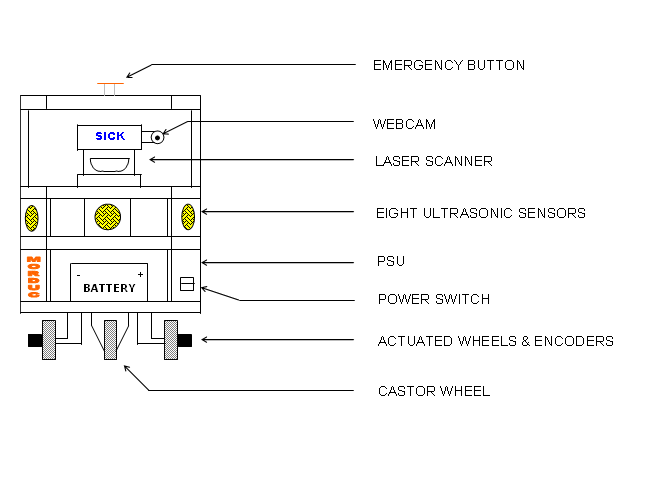
\includegraphics[width=300pt]{img/Morduc_scheme.png}
    \caption{3morduc's schematic figure}
    \label{fig:morduc_scheme}
  \end{center}
\end{figure}
\\
Besides, on the same lower level is located an electronic board
controlling different modules, each one predisposed to manage a
specific task as movements, sensors and communication.
\\
Type and number of sensors avaible on 3morduc are:

\begin{itemize}
\item \texttt{belt of bumpers} \\
  A belt of bumpers (in total 16 switches) is dislocated around
  the entire perimeter on the robot base, just over the wheels level. \\
  See chapter \textit{Bumper} (\ref{sec:mobile:bumper}) for more details
  about this type of sensor.

\item \texttt{incremental encoders} \\
  The two robot motor axes are equipped with incremental encoders, with
  resolution of 500 pulses per turn. These sensors are useful to calculate
  heading and position of the robot by using the kinematic model. \\  
  See chapter \textit{Encoder} (\ref{sec:mobile:encoder}) for more details
  about this type of sensor.
 
\item \texttt{belt of sonars} \\
  On the second level are located eight sonar sensors, which measure the
  distance from an obstacle using the flight time of an ultrasonic signal
  produced by means of a vibrating piezoelectric sensor. \\
  See chapter \textit{Sonar} (\ref{sec:mobile:sonar}) for more details
  about this type of sensor.

\item \texttt{scanner laser} \\
  In order to detect obstacles on the workspace, the \textit{Laser Measurement
  Sensor} (LMS) operates by measuring the flight time of a pulsed laser
  light beam that is reflected by obstacle, to provide a 2D scanning data. \\
  It is possible to configure different angular resolution (0.25\textdegree,
  0.5\textdegree or 1\textdegree pace) with different angular scan (100\textdegree
  or 180\textdegree).
  \begin{figure}[h]
    \begin{center}
      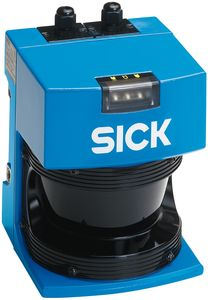
\includegraphics[width=60pt]{img/laser_sick_lms_200.jpg}
      \caption{LMS Sick mounted on 3morduc}
      \label{fig:laser_sick_lms_200}
    \end{center}
  \end{figure}
  \\
  See chapter \textit{Laser} (\ref{sec:mobile:laser}) for more details
  about this type of sensor. The reference manual about \textit{LMS
  Sick 200} can be found at \cite{3morduc:laser_sick_200}.

\item \texttt{stereo cameras} \\
  On the robot there are also two stereoscopic cameras, each one with a
  resolution of 1.3 Megapixel and fixed focus lens of 4.0 mm. \\
  The CCD sensors of these cameras have a good noise immunity and
  sensibility; moreover, it is possible to adjust all the image parameter, e.g.
  exposure gain, frame rate, resolution. \\
  The cameras are mounted on a rigid support; it permits to simply adjust
  the camera distance in a range 5-20 cm. \\
  Both the cameras can be connected to PC by IEEE 1394 interface, with a
  frequency of syncronization of 8 Khz. \\
  \begin{figure}[h]
    \begin{center}
      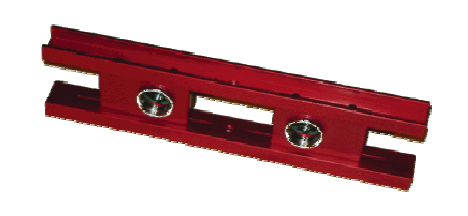
\includegraphics[width=200pt]{img/camera_videre.png}
      \caption{STH-MDCS2-VAR-C mounted on 3morduc}
      \label{fig:camera_videre}
    \end{center}
  \end{figure}
  \\
  See chapter \textit{Image sensors} (\ref{sec:mobile:image}) for more details
  about this type of sensor. The reference manual about the \textit{STH-MDCS2-VAR-C}
  can be found at \cite{3morduc:camera_sth_mdcs2}.

  

\end{itemize}

More images, video and information about 3morduc can
be found at \cite{morduc:features}.


\subsubsection{Internet communication}
\label{sec:3morduc:communication}

How client-server model is implemented.
